\section{The Holy Cross Energy Project}\label{sec:hce}

The initial TESS deployment and field experiment is taking place in partnership with Holy Cross Energy (HCE). The HCE implementation represent a so-called minimum viable product (MVP), and focuses only on new kinds transactive resources, i.e., photovoltaics, batteries, and electric vehicles.  Although supported by TESS, less emphasis is being placed on demand response resources like heat pumps and water heaters.  
In the following section, we describe the setting of Holy Cross Energy and their motivation to deploy a TS (\cref{sec:HCE_description}), the Basalt Vista project (\cref{sec:Basalt}), and their existing tariff structure (\cref{sec:HCE_tariff}). 

\subsection{Holy Cross Energy}\label{sec:HCE_description}

Holy Cross Energy (HCE) is a member-owned electric cooperative in Colorado. Its service territory includes the Roaring Fork Valley from Aspen to Glenwood Springs, and the Eagle River and Colorado River Valleys from Parachute to Vail, as seen in \cref{fig:HCE_service_territory}. It provides power to over 57,000 premises and operates around 3,000 miles of transmission and distribution lines, with a summer peak of 150 MW. HCE's members are predominantly residential, small commercial, and ski resorts. 

\begin{figure}[t]
\centering
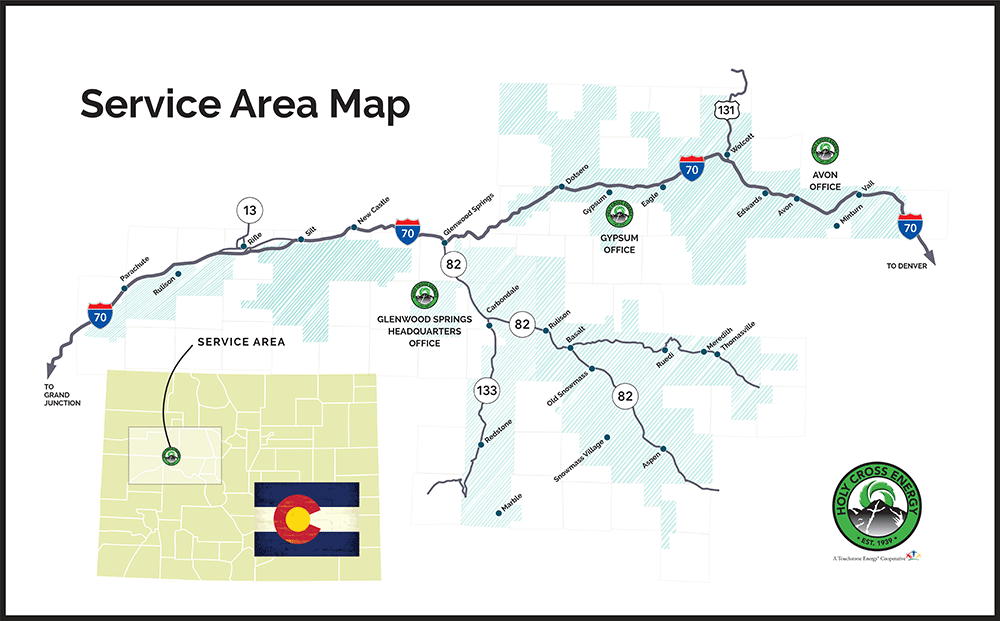
\includegraphics[scale=0.4]{HolyCrossEnergy-Service-Area-Map.png}
\caption{HCE Service Territory}
\label{fig:HCE_service_territory}
\end{figure}

HCE's load during peak periods is dominated by winter resort activity, i.e., residential and lodging loads, along with day-time winter sports and night-time snow making.  The residential and lodging loads are not sufficiently flexible to participate greatly in demand response (DR) programs. However, HCE has put in place a number of DR programs that resorts participate in should load-shedding be required, particularly for those relating to night-time snow-making demand.

HCE purchases most power on long-term contracts with Public Service Company of Colorado (an Xcel Energy company) and the Western Area Power Association. The price of electricity under the long-term contract is \$0.02/kWh but increases to \$13/kW during the monthly coincident peak, i.e. the peak of the Xcel service territory. HCE's annual peaks usually occur in late December and early January during the holiday season. The 2018 summer peak was 156.3 MW and the winter peak was 256.3 MW.  In 2018 net generation was 461 GWh and wholesale procurement was 774 GWh with retail sales of 1,233 GWh.

Furthermore, HCE is considering participating in the Western Electric Coordinating Council (WECC) energy balancing market, as part of a broader agreement between Xcel and the Western EIM operated by CAISO \citep{CAISO2020}. Under this agreement, HCE would be exposed to real-time wholesale market prices at which it could buy or sell electricity. Increased demand flexibility would enable HCE to manage its load, revenue, and costs more actively.

With regard to emissions, in 2019 HCE's fuel mix was 44 percent renewable, 40 percent coal, and 7 percent natural gas, and the remainder is unknown \citep{HCE2019}. The renewable resources are mainly wind (31 percent), biomass (7 percent), and hydro (3 percent), with the remainder solar and mine methane. HCE has an ambitious carbon reduction target of having a greenhouse gas emission-free fuel mix by 2030. In 2018 HCE set a target of 70 percent greenhouse gas emission-free by 2030, and subsequent improvements in clean energy technologies have led them to revise the target to 100 percent by 2030. To meet this goal, HCE is investing in infrastructure to increase its adoption of technologies like electric vehicles, rooftop solar PV, and storage, as well as digitization to interconnect DERs and optimize their dispatch. 

Resilience is another priority for HCE, particularly against wildfire risk. In 2018, the Lake Christine wildfire spread in the Roaring Fork Valley, causing the evacuation of thousands in Carbondale, El Jebel, Basalt, and Fryingpan Valley, and destroying over 12,000 acres. In a mountainous region with abundant large wildlife and a single transmission line, HCE faces considerable technical challenges in achieving a resilient high-DER system. Increasing DER adoption and digital interconnection will provide flexibility that contributes to resilience, and the coordination using price-based dispatch through TESS enables that flexibility.

\subsection{Basalt Vista}\label{sec:Basalt}

To learn more about DER management and to experiment with involving customers in sustainable system management, HCE and other community partners are collaborating with Habitat for Humanity to construct affordable housing in Basalt and equip it with digital and DER-enabling infrastructure. Each of the 27 houses will have solar PV, EV charging, and hookups for battery storage. The houses in the community are connected to each other and capable of autonomous energy sharing using the National Renewable Energy Laboratory's Network Optimized Distributed Energy Systems (NODES) algorithm \citep{IEEESpectrumNREL}. 

TESS is part of the larger Basalt Vista project, a collaboration between the Roaring Fork School District, which donated the land, Pitkin County, which funded the road and utilities, and Habitat for Humanity, which raised the funds to cover the gap between the costs to build the homes and the revenue from the purchase prices, as well as facilitating mortgage access and assistance.  The Community Office for Resource Efficiency helped fund the high-performance heating and photovoltaic systems, and Holy Cross Energy donated the inverters, electric vehicle chargers, hot water heaters, controllers, and the batteries for the first four homes.  Additional financial support and discounts were provided by the vendors, including Bryant Colorado, Sunsense Solar, the Town of Basalt, LE, and a number of private donors. The TESS team was invited to deploy controllers in the first four houses with the goal of implementing a full Type 2.0 TS using the TESS platform, connected to operations with a newly-designed control room display. The TESS deployment in Basalt Vista aims to help HCE reduce procurement cost, decrease carbon emissions, and improve resilience capabilities. The project is supported financially by the Department of Energy's Office of Electricity from October 2019 through September 2021.

\subsection{Existing Tariff System}\label{sec:HCE_tariff}

In the HCE implementation, one important market design requirement is that TESS complements HCE's existing residential retail tariff \citep{holy_cross_energy_electric_2020}.
\cref{tab:HCE-tariff} summarizes the terms of the residential rate options available to HCE members who own DERs. All residential customers start with a base rate tailored to the size of their home and its electricity consumption profile. They can also choose a time of use rate with lower off-peak and higher peak energy charges. 

\begin{table}[t]
\centering
\caption{Holy Cross Energy Residential Rate Tariff}
\label{tab:HCE-tariff}
\begin{tabular}{@{}lll@{}}
\toprule
\textbf{Rate}                                                                        &                                                                                      & \textbf{Terms}                                                                                                                                      \\ \midrule
\textit{\begin{tabular}[c]{@{}l@{}}Residential \\ Services\end{tabular}}             & Small Base                                                                           & \begin{tabular}[c]{@{}l@{}}Monthly consumer charge \$12, \\ energy charge \$0.105/kWh\end{tabular}                                                    \\ \cline{2-3}
                                                                                     & Large Base                                                                           & \begin{tabular}[c]{@{}l@{}}Monthly consumer charge \$28, \\ demand charge \$5.32/kW,\\ energy charge \$0.077/kWh\end{tabular}                         \\ \cline{2-3}
                                                                                     & \begin{tabular}[c]{@{}l@{}}Time of Use \\ (TOU)\end{tabular}                         & \begin{tabular}[c]{@{}l@{}}Monthly consumer charge \$12, \\ off-peak energy charge \$0.06/kWh,\\ peak energy charge \$0.24/kWh (4pm-9pm)\end{tabular} \\ \midrule
\textit{\begin{tabular}[c]{@{}l@{}}Net Energy \\ Metering (NEM)\end{tabular}}      &                                                                                      & \begin{tabular}[c]{@{}p{8cm}}On-premise generation offset at HCE's retail rate/kWh\end{tabular}                                    \\
                                                                                     &                                                                                      & \begin{tabular}[c]{@{}p{8cm}}Settlement calculated and payment made annually for excess generation at cost\end{tabular}                                                                    \\ \midrule
\textit{\begin{tabular}[c]{@{}l@{}}Distribution \\ Flexibility Pricing\end{tabular}} & \begin{tabular}[c]{@{}l@{}}Distribution \\ Flexibility \\ Program (DFP)\end{tabular} & \begin{tabular}[c]{@{}p{8cm}}Bill credit, amount based on agreed measurement and demand response performance\end{tabular}                       \\ \cline{2-3}
                                                                                     &                                                                                      & Customer grants DER control to HCE                                                                                                                  \\
                                                                                     &                                                                                      & HCE receives attributes, e.g., RECs                                                                                                                 \\
                                                                                     & \begin{tabular}[c]{@{}l@{}}Peak Time Rebate \\ Program (PTR)\end{tabular}            & \begin{tabular}[c]{@{}p{8cm}}Bill credit for actual measured reduction\end{tabular}                                                                \\
                                                                                     &                                                                                      & \begin{tabular}[c]{@{}p{8cm}}\$1/kWh during Critical PTR, \$0.50/kWh during High PTR\end{tabular} 
                                                                                                          \\ \midrule
\textit{\begin{tabular}[c]{@{}l@{}}DER Service \\ Agreement\\ (DERSA)\end{tabular}}  &                                                                                      & \begin{tabular}[c]{@{}p{8cm}}HCE pays most of initial DER cost, and recoups that cost through monthly amortized customer payments\end{tabular}   \\
                                                                                     &                                                                                      & Customer grants DER control to HCE                                                                                                                  \\
                                                                                     &                                                                                      & \begin{tabular}[c]{@{}p{8cm}}DER payments are on Net Energy Metering terms\end{tabular}                                                            \\
                                                                                     &                                                                                      & \begin{tabular}[c]{@{}p{8cm}}DERSA customers thus are \\ automatically on DFP\end{tabular}                             \\ \bottomrule
\end{tabular}

\end{table}

If they own one or more DERs, customers can opt into the net energy metering (NEM) rate, under which they pay the retail rate only on their net consumption. Their own generation substitutes for grid-supplied generation, so when their generation is less than their consumption, its value is the relevant retail rate, which is substantially higher than if they were paid the applicable procurement price for electricity. At the end of the year NEM customers are paid HCE's bulk supply procurement rate for any excess net generation they may have produced.

Moreover, HCE's Distribution Flexibility Pricing offers two additional programs: the Distribution Flexibility Program (DFP) and the Peak Time Rebate Program (PTR). The Distribution Flexibility Program (DFP) provides a bill credit for demand response performance, in return for granting HCE operational control for occasional load cycling and for outage control, for instance, during emergency situations or during a forecasted coincident peak. If the DER's generation has any environmental attributes (e.g., renewable energy certificates or RECs) or tax benefits, HCE receives those attributes and their benefits.

The PTR program provides bill credits for measured demand reduction during peak events. An example of such an event is the Xcel system-wide coincident peak, during which HCE pays significantly higher procurement costs (see \cref{sec:HCE_description}). HCE members receive a \$1.00/kWh PTR bill credit for actual consumption reduction during Critical PTR events, and a \$0.50/kWh credit during High PTR events, including high-demand winter periods. In 2020 most PTR events took place between 4PM and 9PM, lasted 2-3 hours, and were limited to a maximum of 96 hours per year. PTR events were declared one day ahead, but could be scheduled the same day if necessary, with notice being provided electronically or on HCE's websites. The expected consumer baseline is based on historical consumption, with no penalty for failure to reduce consumption.

An additional program supports member expenditures to install DERs and let them benefit from using DERs to bring flexibility to the distribution system. Under this DER Service Agreement (DERSA), customers can choose to purchase their DERs through HCE, with HCE paying most of the initial costs and then charging the customer a monthly amortized payment to recoup that cost over time. The DER investment is more affordable, and in return the customer grants operational control to HCE. DERSA customers also receive NEM compensation for excess generation. If the DER's generation has any environmental attributes (e.g., renewable energy certificates or RECs) or tax benefits, HCE receives those attributes and their benefits. 

Under the current tariff, Basalt Vista customers are not subject to DERSA or DFP/PTR because HCE donated the assets. Instead, they are subject to direct control by HCE (as under DFP, but without the financial aspect). 





